\documentclass{report}
\usepackage[utf8]{inputenc}
\usepackage[margin=1in]{geometry}
\usepackage{array}
\usepackage{multirow}
\usepackage{makecell}
\usepackage{listings}
\usepackage{pdflscape}
\usepackage{longtable}
\usepackage{indentfirst}
\usepackage{multicol}
\usepackage{graphicx}
\graphicspath{ {images/} }
\setlength{\columnsep}{1cm}

\title{Schwap CPU}
\author{Team M: \\ Charlie Fenoglio, Alexander Hirschfeld, \\ Andrew McKee, and Wesley Van Pelt}
\date{Winter 2015/2016}

\begin{document}
\maketitle
\setcounter{tocdepth}{4}
\tableofcontents

\chapter{Report}
	\section{Executive summary}
		The Schwap CPU is a load/store style CPU architecture that features 64 schwappable registers, kernel and userspace, a stack, and ports for IO devices. The Schwap CPU comes with a simplistic compiler, an assembler, a program loader for the creation of COE memory files, and an emulator for improving development workflows. The Schwap CPU comes with a myriad of example programs and a basic kernel for simplifying the process of learning and developing for the Schwap CPU. In the future the Schwap CPU team hopes to add a more complex compiler, extend the CPU to support and handle hardware exceptions, and add the hardware to use the IO on the Spartan E3 board.
	\section{Introduction}
		Welcome to the Schwap CPU.  This is new age 16-bit CPU that will solve all of performance problems.  We have a new innovative way of handling the limitations of the 16-bit limit on the instructions size of this architecture with the only downside being the clock speed of our clock! With all of the new registers you programmers will never need to touch the slow, evil memory more than once per instruction cycle. There are also Input/Output capabilities! So what are you waiting for, get schwapping!
	\section{Body}
		\subsection{Instruction Set Design}
			Our assembly design was built around the idea that an accumulator can best use a 16 bit instruction.  In MIPS, there are 15 bits set aside for all of the declaration that MIPS needs for directing data to the correct register. When looking through what we needed and wanted to accomplish we chose a design that would reuse the first source register as the destination register. This design choice was also seen in the IA-32. Because we are using 8 of the 16 bits of the instruction, we are able to have 4 bits for our function code, and another 4 bits for anything else.\par
			The 4 bits at the end of the instruction are used to declare the operation for the ALU and as an unsigned offset for branching and read/write., The ALU ops code being the last 4 bits of the instruction allows us to have all of the common ALU operations and a few extra with the option of adding more if we should ever need. We also decided that the best way to handle immediate loading would be to have a dual port RAM. This enables us to load immediates immediately without using multiple instructions or additional instructions. All of the immediate loading is done through the ALU operations because we determined that the majority of immediates used will be while doing mathematical operations.\par
			The unsigned offsets for branching and read/writes forces the programmer to think before they write code create more optimized code, and creating code that is easier to read. Knowing that branches can only move down creates an environment that is much easier to debug after the code has been assembled to hex. One of the downsides to this is that the assembler must be more complex to account for branching up and down, as well as branching over more than 16 instructions. There is luckily a clever way to handle this by inverting the checked conditions and branching over a jump to the new destination. The other limiting thing with the 4 bit unsigned offset comes from read and write. The programmer is only able to read or write 16 places above the current memory address, this limitation is something that will have to be worked around by the programmers because unlike branching, the Assembler does not handle converting a number above 15 as a pseudo instruction.\par
			Another limited thing is jumping. Jumps have an 8 bit signed offset from the starting address passed to them. This gives jumps a range of -128 lines to 127 lines above or below the address in the register. Normal jumps are done based on PC, however any register will work. This decision was made because we wanted to encourage the use of PC relative jumps in methods to allow them to be more portable after they have been assembled. The assembler can handle jumping outside of the range, there is no good practice for doing this by hand outside of knowing the exact location in memory for which the programmer wants to jump, loading that into a temporary value, and using that as the register outside of offset.\par
			To get around the limitation of 16 registers, we decided to implement a set of registers called "Schwap". These 16 sets of 4 registers are accessed in sets of 4. These registers behave exactly the same as the other registers when they are selected, however they can be ‘stored’ or deselected with a command and another set of 4 brought into the positions of the previous. The stored values, outside of special values for IO, cannot change. These swappable registers are our solution to passing arguments, IO, and extending the users working variables so they do not have to use memory as often.\par
			IO is based out of schwap 11. The way this was designed, we have two buses that pass out of the schwap module that overrides the registers that would be written to or read from. This allows us to handle writing to an IO device and reading from it without having to deal with exceptions. This unfortunately does not let us have code that will run every time a button is pressed unless the programmer explicitly has code wait for a button. Because there are seperate buses for reading from and writing two IO, we do not have to deal with bidirectional wires and the inconsistency that they would have created. Schwap 11 has 4 registers allocated to it. These are laid out as: \$h0; port 1, \$h1. data 1, \$h2 port 2, \$h3; data 2. This allows us to declare and use two IO devices at once. There are two clock signals that are also passed out of the Schwap, one is high for one cycle after the schwap register is read from, and the other is high for one cycle during a write, and for part of a tick before the write happens. This is to allow time for the IO devices to prepare for the write, or reset after a read if they are accumulators. This is implemented in the HDL and in the datapath, but we do not have the Verilog to support this on the board itself.
		\subsection{Xilinx Implementation}
			Everything that was done in Xilinx was done with Verilog code rather than schematics. This was done to more easily merge files and track what changes were made between versions. This turned out to be a benefit because Verilog code is easy to understand and modify and has a find a replace functionality.  One of the downsides to using Verilog is that we don't have control over what decisions the HDL compiler makes. We cannot chose to optimize things by using a less efficient pattern on silicon that has a faster throughput.\par
			We broke things down into what we determined to be the most efficient patterns: Memory and PC, the ALU, Schwap, and Control. These were then combined into larger groups, Register file, containing Schwap and other logic, and then the Register file and ALU. Each of these components were tested independently before we attached everything together. One of the things that we found is that separate testing does not let us account for timing errors that happened when we had things chained together.
		\subsection{Testing Methodology}
			With each component, we tested to make sure that it functioned as intended. These tests did not cover every single combination, but they did cover all edge cases and common cases that we thought would appear most frequently. These tests were mostly used to make sure that the part functioned correctly and would continue to function correctly as we attached the components together and modified timings and add to the components and modified the RTL to suite the ever changing needs that we found or created.\par
			As we created new elements to add to the data path, we started by defining what we thought the results should be then built a component that complied with what we defined before starting. This let us start writing tests before component was finished or started.
		\subsection{Final Results}
			Using the XST Synthesis we tested the maximum possible performance. According to these calculations, our CPU has an approximate maximum frequency of 30 MHz, executing a cycle in about 33.3ns. On average for the RelPrime program, each instruction takes about 2.5 cycles. With a total of 45,115 instructions, the program runs in 3.759ms total time. The total storage space used for RelPrime and Euclid's Algorithm is 76 bytes.
	\section{Conclusion}
		Now that you are having fun with your new Schwap CPU and have learned about some of the design decisions of the engineering team behind the brilliance of this Computational Processing Unit, feel just shout and curse if you are having problems getting things to work correctly. I know the team was. If you call +1 (812) 877-8396 now, we will provide the broken code for the IO, and a hardly working assembler/compiler so you can work hard to get them to work too! Current price the only minimum wage for about 375 man hours worth of college student time, blood, sweat, and tears.
\chapter{Design Documentation}
	\section{Registers}
	There are a total of 76 16-bit registers; 12 are fixed and 64 (spilt into 16 groups of 4) "schwapable" registers.  Some registers have alias names, see Section 11.3.1 for a list.
	\subsection{Register Names and Descriptions}
		\begin{center}
			\begin{tabular}{| c | c | c | c |} \hline
				Name        & Number  & Description            & Saved Across Call? \\ \hline
				\$z0        & 0       & The Value 0$^\dagger$  & -   \\ \hline
				\$a0        & 1       & Assembler Temporary 0  & No  \\ \hline
				\$a1        & 2       & Assembler Temporary 1  & No  \\ \hline
				\$pc        & 3       & Program Counter$^\dagger$&Yes\\ \hline
				\$sp        & 4       & Stack Pointer          & Yes \\ \hline
				\$ra        & 5       & Return Address         & Yes \\ \hline
				\$s0 - \$s1 & 6 - 7   & User Saved Temporaries & Yes \\ \hline
				\$t0 - \$t3 & 8 - 11  & User Temporaries       & No  \\ \hline
				\$h0 - \$h3 & 12 - 15 & Schwap                 & -   \\ \hline
			\end{tabular} \\
			$^\dagger$See Section 2.11.1.1-1 for details
		\end{center}
	\subsection{Schwap Registers}
		The "schwap" registers are registers that appear to be swapped using a command.  There is no data movement when schwapping, it only changes which registers the \$h0 - \$h3 refer to.  There are 8 groups the user can use for general purpose and 8 reserved groups.
		\subsubsection{Schwap Group Numbers, Descriptions, and Uses}
			\begin{center}
				\begin{tabular}{| c | c | c | c |} \hline
					Group Number & ID    & Uses                      & Saved Across Call? \\ \hline
					0 - 3        & 0 - 3 & User Temporaries          & No \\ \hline
					4 - 7        & 0 - 3 & User Saved Temporaries    & Yes\\ \hline
					8            & 0 - 3 & Arguments 0 - 3           & No \\ \hline
					9            & 0 - 3 & Return Values 0 - 3       & No \\ \hline
					\multirow{4}{*}{10} & 0 & The constant 1         & -  \\ \cline{2-4}
					             & 1     & The constant -1           & -  \\ \cline{2-4}
					             & 2     & The constant 42           & -  \\ \cline{2-4}
					             & 3     & The constant 1337         & -  \\ \hline
					\multirow{4}{*}{11} & 0 & Port number for device 0 & -\\ \cline{2-4}
					             & 1     & I/O for device 0          & -  \\ \cline{2-4}
					             & 2     & Port number for device 1  & -  \\ \cline{2-4}
					             & 3     & I/O for device 1          & -  \\ \hline
					12           & 0 - 3 & Sudo values 0 - 3         & No \\ \hline
					13           & 0 - 3 & Kernel Reserved           & -  \\ \hline
					14 - 15      & 0 - 3 & Illuminati Reserved       & -  \\ \hline
				\end{tabular} \\
			\end{center}
\section{Instructions}
	All instructions are 16-bits.  The destination register is also used as a source unless otherwise noted.
	\subsection{Instruction Types and Bit Layouts}
		Instructions can be manually translated by putting the bits for each of the components of the instructions in the places listed by the diagrams for each type.  The OP and function codes can be found in section 2.2.2.  The destination and source are register numbers, which can be found under the "Register Names and Descriptions" (1.1) table.  Schwap group numbers can be found under the "Schwap Group Numbers, Descriptions, and Uses" (2.1.2) table.  The active schwap group and sudo code number is not preserved over a function call.
		\subsubsection{A-Type}
			\begin{center}
				\begin{tabular}{l r l r l r l r}
					\hline
					\multicolumn{2}{| p{2cm} |}{OP Code} & \multicolumn{2}{p{2cm}}{Destination} & \multicolumn{2}{| p{2cm} |}{Source} & \multicolumn{2}{p{2cm} |}{Func. Code} \\ \hline
					15 & 12 & 11 & 8 & 7 & 4 & 3 & 0
				\end{tabular}
				\begin{tabular}{l r l r l r l r}
					\hline
					\multicolumn{2}{| p{2cm} }{Immediate} & \multicolumn{2}{p{2cm}}{ } & \multicolumn{2}{ p{2cm} }{ } & \multicolumn{2}{p{2cm} |}{ } \\ \hline
					15 & & & & & & & 0
				\end{tabular}
			\end{center}
			Used for all ALU operations.  It consists of a 4-bit OP code, 4-bit destination, 4-bit source, and a 4-bit function code.  If the instruction has an immediate, it is inserted as the next instruction, and if a source is not given then it should be all 0's.
		\subsubsection{B-Type}
			\begin{center}
				\begin{tabular}{l r l r l r l r}
					\hline
					\multicolumn{2}{| p{2cm} |}{OP Code} & \multicolumn{2}{p{2cm}}{R0} & \multicolumn{2}{| p{2cm} |}{R1} & \multicolumn{2}{p{2cm} |}{Offset} \\ \hline
					15 & 12 & 11 & 8 & 7 & 4 & 3 & 0
				\end{tabular}
			\end{center}
			If it is being used for branching it consists of a 4-bit OP code, 4-bit 1st source (R0), 4-bit 2nd source (R1), and a 4-bit (unsigned) offset. If it is being used for reading from memory it consists of a 4-bit OP code, 4-bit destination (R0 not used as a source), 4-bit source (R1, it is a memory address), and a 4-bit (unsigned) offset.  If it is being used for writing to memory it consists of a 4-bit OP code, 4-bit source (R0), 4-bit destination (R1, it is a memory address), and a 4-bit (unsigned) offset.  R0 and R1 are registers.
		\subsubsection{H-Type}
			\begin{center}
				\begin{tabular}{l r l r l r l r}
					\hline
					\multicolumn{2}{| p{2cm} |}{OP Code} & \multicolumn{2}{p{2cm}}{ } & \multicolumn{2}{p{2cm}}{ } & \multicolumn{2}{| p{2cm} |}{Group} \\ \hline
					15 & 12 & & & & & 3 & 0
				\end{tabular}
			\end{center}
			Used for schwapping and sudo.  It consists of a 4-bit OP code, 8 unused bits, and a 4-bit schwap group number or sudo use case which are immediates.
		\subsubsection{J-Type}
			Used for jumping.  It consists of a 4-bit OP code, 4-bit source register, and an 8-bit (signed) offset.
			\begin{center}
				\begin{tabular}{l r l r l r l r}
					\hline
					\multicolumn{2}{| p{2cm} |}{OP Code} & \multicolumn{2}{p{2cm}}{Source} & \multicolumn{2}{| p{2cm} }{Offset} & \multicolumn{2}{p{2cm} |}{ } \\ \hline
					15 & 12 & 11 & 8 & 7 & & & 0
				\end{tabular}
			\end{center}
	\subsection{Core Instructions}
		Some instructions have alias names, see Section 2.11.3 for a list. [dest], [src], [src0], [src1] all refer to a register in the register file, for example \$t0.  "NAM" stands for the name of the instruction (for example, "and").  "OP" stands for whatever the op would be (for example, "\&").
		\subsubsection{A-Type}
			\begin{center} \begin{tabular}{| c | c | c |} \hline
				\thead{Function \\ Code} & Name & Description \\ \hline
				0x0 & and & \thead{Bitwise ands 2 values}\\ \hline
			    0x1 & orr & \thead{Bitwise ors 2 values}\\ \hline
			    0x2 & xor & \thead{Bitwise xors 2 values}\\ \hline
			    0x3 & not & \thead{Bitwise nots the first value}\\ \hline
			    0x4 & tsc & \thead{Converts a number to 2's compliment}\\ \hline
			    0x5 & slt & \thead{Set less than}\\ \hline
			    0x6 & sgt & \thead{Set greater than}\\ \hline
			    0x7 & sll & \thead{Left logical bit shift}\\ \hline
			    0x8 & srl & \thead{Right logical bit shift}\\ \hline
			    0x9 & sra & \thead{Right arithmetic bit shift}\\ \hline
			    0xA & add & \thead{Adds 2 values}\\ \hline
			    0xB & sub & \thead{Subtracts 2 values}\\ \hline
			    0xF & cpy & \thead{Copies the value in one register to another}\\ \hline
			\end{tabular} \end{center}
			All A-Type instructions, except for not, tsc, slt, and cpy, follow the syntax in the first section of the table below.  Those three can be found in the next sections.
			\begin{center} \begin{tabular}{| c | l | c | c |} \hline
				\thead{OP\\Code}     & Syntax                       & Meaning & Description \\ \hline
				0x0                  & NAM [dest] [src]             & \thead{dest $=$ dest OP src} & \thead{OPs the values in registers [dest] and [src]}\\ \hline
				\multirow{3}{*}{0x1} & NAM [dest] [src] [immediate] & \thead{src $=$ immediate \\ dest $=$ dest OP src} & \thead{Loads the immediate into the register [src] and \\ then OPs the values in registers [dest] and [src]}\\ \cline{2-4}
				                     & NAM [dest] [immediate]       & \thead{dest $=$ dest OP immediate} & \thead{OPs the immediate and the value in the \\ register [dest]}\\ \hline \hline
				0x0                  & not [dest]                   & \thead{dest $=$ $\sim$dest} & \thead{Bitwise nots the value in the register [dest]}\\ \hline
				0x0                  & tsc [dest]                   & \thead{dest $=$ $\sim$dest + 1} & \thead{Converts the value in the register [dest]\\to 2's compliment}\\ \hline
				0x1                  & tsc [dest] [src] [immediate] & \thead{src $=$ immediate \\ dest $=$ $\sim$src + 1} & \thead{Loads the immediate into the register [src] \\ and then converts the value in register [src] \\ to 2's compliment and stores into [dest]}\\ \cline{2-4}
				0x0                  & slt [dest] [src]             & \thead{dest $=$ (dest $<$ src) ? 1 : 0} & \thead{If [dest] $<$ [src], then [dest] gets set to 1 \\ If [dest] $\geq$ [src], then [dest] gets set to 0}\\ \hline
				\multirow{3}{*}{0x1} & slt [dest] [src] [immediate] & \thead{src $=$ immediate \\ dest $=$ (dest $<$ src) ? 1 : 0} & \thead{Loads the immediate into the register [src] then \\ If [dest] $<$ [src], then [dest] gets set to 1 \\ If [dest] $\geq$ [src], then [dest] gets set to 0}\\ \cline{2-4}
						             & slt [dest] [immediate]       & \thead{dest $=$ \\ (dest $<$ immediate) ? 1 : 0} & \thead{If [dest] $<$ [immediate], then [dest] gets set to 1 \\ If [dest] $\geq$ [immediate], then [dest] gets set to 0}\\ \hline \hline
				0x0                  & cpy [dest] [src]             & \thead{dest $=$ src} & \thead{Copies the value the in register [src] into [dest]}\\ \hline
				0x1                  & cpy [dest] [immediate]       & \thead{dest $=$ immediate} & \thead{Loads the immediate into the register [dest]}\\ \hline
			\end{tabular} \end{center}
		\subsubsection{B-Type}
			\begin{center} \begin{tabular}{| c | c | c |} \hline
				\thead{OP \\ Code} & Name & Description \\ \hline
				 0x2 & beq  & \thead{Branches if the 2 values are equal}\\ \hline
				 0x3 & bne  & \thead{Branches if the 2 values are not equal}\\ \hline
				 0x4 & bgt  & \thead{Branches if value0 $>$ value1}\\ \hline
				 0x5 & blt  & \thead{Branches if value0 $<$ value1}\\ \hline
				 0x7 & r    & \thead{Reads the value in memory into a register}\\ \hline
				 0x8 & w    & \thead{Writes the value in a register into memory}\\ \hline
			\end{tabular} \end{center}
			The four different types of branches all follow the same syntax, "bnh" represents any branch name and "***" represents the condition.  They will become pseudo instructions iff branching up, or down more than 16 instructions.  Read and write each have their own syntaxes.  [offset] is not a register, it is an immediate.
			\begin{center} \begin{tabular}{| l | c | c |} \hline
				Syntax & Meaning & Description \\ \hline
				bnh [src0] [src1] label  & \thead{if(src0 *** src1) goto label} & \thead{If [src0] *** [src1], branch to label}\\ \hline
				r [dest] [offset]([src]) & \thead{dest $=$ Mem[src + offset]} & \thead{Reads the data in the address of [src] + [offset] \\ in memory into [dest]}\\ \hline
				w [offset]([dest]) [src] & \thead{Mem[dest + offset] $=$ src} & \thead{Writes the data in the address of [dest] + [offset] \\ in memory from [src]}\\ \hline
			\end{tabular} \end{center}
		\subsubsection{H-Type}
			\begin{center} \begin{tabular}{| c | c | l | c |} \hline
				\thead{OP \\ Code} & Name & Syntax & Description \\ \hline
				 0xA & scp  & scp         & \thead{Switches PC to user PC from kernel PC}\\ \hline
				 0xE & rsh  & rsh [group] & \thead{Changes the schwap group number to [group], \\ these numbers can be found in the table in 1.2.1}\\ \hline
				 0xF & sudo & sudo [code] & \thead{Similar to syscall in MIPS, see kernel \\ documentation for details} \\ \hline
			\end{tabular} \end{center}
		\subsubsection{J-Type}
			\begin{center} \begin{tabular}{| c | c | l | c | c |} \hline
				\thead{OP \\ Code} & Name & Syntax & Meaning & Description \\ \hline
				 0x6 & jr & jr [dest] [offset] & \thead{pc $=$ dest + offset} & \thead{Jumps to the instruction at the address in [dest] + [offset]}\\ \hline
			\end{tabular} \end{center}
	\subsection{Pseudo Instructions}
		There are two types of pseudo instructions.  One are instructions which are always pseudo instructions, the other are sometimes pseudo depending on the conditions.  Some instructions have alias names, see Section 2.11.3 for a list.
		\subsubsection{Always Pseudo Instructions}
			\begin{center} \begin{tabular}{| c | c | c | c |} \hline
				Name & Syntax    & Actual Code & Description \\ \hline
				j    & j label   & \thead{cpy \$a0 [label pc] \\ jr \$a0 0} & \thead{Jumps to the instruction at label}\\ \hline
				jal  & jal label & \thead{cpy \$ra \$pc \\ j [label]} & \thead{Stores the return address and then jumps to the label} \\ \hline
				bge  & bge [src0] [src1] label & \thead{cpy \$a0 [src0] \\ slt \$a0 [src1] \\ beq \$a0 \$z0 label} & \thead{If [src0] $\geq$ [src1], branch to label} \\ \hline
				ble  & ble [src0] [src1] label & \thead{cpy \$a0 [src1] \\ slt \$a0 [src0] \\ beq \$a0 \$z0 label} & \thead{If [src0] $\leq$ [src1], branch to label} \\ \hline
			\end{tabular} \end{center}
		\subsubsection{Conditional Pseudo Instructions}
			\begin{center} \begin{tabular}{| c | c | c | c |} \hline
				Name & Syntax                    & Actual Code & Condition \\ \hline
				beq  & beq [src0] [src1] label & \thead{bnq [src0] [src1] Next \\ j label \\ Next:} & \thead{Branching up or branching down \\ more than 16 instructions}\\ \hline
				bne  & bne [src0] [src1] label & \thead{beq [src0] [src1] Next \\ j label \\ Next:} & \thead{Branching up or branching down \\ more than 16 instructions}\\ \hline
				bgt  & bgt [src0] [src1] label & \thead{blt [src0] [src1] Next \\ j label \\ Next:} & \thead{Branching up or branching down \\ more than 16 instructions}\\ \hline
				blt  & blt [src0] [src1] label & \thead{bgt [src0] [src1] Next \\ j label \\ Next:} & \thead{Branching up or branching down \\ more than 16 instructions}\\ \hline
			\end{tabular} \end{center}
	\subsection{Sudo}
		Sudo is the analogous to "syscall" in MIPS.  It does a bunch of system stuff based on the code you give it.
		\begin{center} \begin{tabular}{| c | c |} \hline
			\multicolumn{2}{|c|}{Sudo modes} \\ \hline
			Syntax  & Description \\ \hline
			sudo 0  & \thead{Signifies the end of a program}\\ \hline
			sudo 10 & \thead{Print all kernel registers}\\ \hline
			sudo 11 & \thead{Multiply \$h0 and \$h1 in the kernel schwap}\\ \hline
			sudo 13 & \thead{Push schwap (group number in kernel schwap \$h0) to stack}\\ \hline
			sudo 14 & \thead{Pop schwap (group number in kernel schwap \$h0) from stack}\\ \hline
			sudo 15 & \thead{Self destruct}\\ \hline
		\end{tabular} \end{center}
\section{RTL and Datapath}
	\subsection{Components}
		\subsubsection{Single 16-bit Register}
			\begin{center} \begin{tabular}{| l | l | c |} \hline
				I/O & Name & Size \\ \hline
				In  & in  & 16 \\ \hline
				Out & out & 16 \\ \hline
				Control & write & 1 \\ \hline
			\end{tabular} \end{center}
			\begin{center} \begin{tabular}{| l | c |} \hline
				\multicolumn{2}{|c|}{Used as:} \\ \hline
				IR       & \thead{Stores the 16-bit instruction that comes from memory} \\ \hline
				NextInst & \thead{Stores the next 16-bit instruction that comes from memory} \\ \hline
				ALUout   & \thead{Stores the value that comes out of the ALU} \\ \hline
				MemRead  & \thead{Same as IR, but is used for values} \\ \hline
			\end{tabular} \end{center}
		\subsubsection{Single 4-bit Register}
			\begin{center} \begin{tabular}{| l | l | c |} \hline
				I/O & Name & Size \\ \hline
				In  & in   & 4 \\ \hline
				Out & out  & 4 \\ \hline
				Control & writable & 1 \\ \hline
			\end{tabular} \end{center}
			\begin{center} \begin{tabular}{| l | c |} \hline
				\multicolumn{2}{|c|}{Used as:} \\ \hline
				SchLatch & \thead{Stores schwap group number} \\ \hline
			\end{tabular} \end{center}
		\subsubsection{SE}
			\begin{center} Sign extends \end{center}
			\begin{center} \begin{tabular}{| l | l | c |} \hline
				I/O & Name & Size \\ \hline
				In  & in   & * \\ \hline
				Out & out  & * \\ \hline
			\end{tabular} \end{center}
		\subsubsection{16-bit Adder}
			\begin{center} \begin{tabular}{| l | l | c | l |} \hline
				I/O & Name     & Size & Description \\ \hline
				In  & A        & 16   & First input \\ \hline
				In  & B        & 16   & Second input \\ \hline
				Out & R        & 16   & Result \\ \hline
			\end{tabular} \end{center}
		\subsubsection{ALU}
			\begin{center} \begin{tabular}{| l | l | c | l |} \hline
				I/O & Name     & Size & Description \\ \hline
				In  & A        & 16   & First input \\ \hline
				In  & B        & 16   & Second input \\ \hline
				Out & R        & 16   & Result \\ \hline
				Out & zero     & 1    & If result is 0 \\ \hline
				Out & eq       & 1    & If A $==$ B \\ \hline
				Out & lt       & 1    & If A $<$ B \\ \hline
				Out & gt       & 1    & If A $>$ B \\ \hline
				Control & op   & 4    & Operation code \\ \hline
			\end{tabular} \end{center}
		\subsubsection{PC}
			\begin{center} \begin{tabular}{| l | l | c | l |} \hline
				I/O & Name      & Size & Description \\ \hline
				In  & PCSrc     & 16   & What the PC should be changed to \\ \hline
				Out & PCOut     & 16   & The PC value \\ \hline
				Control&PCWrite & 1    & Set the PC to PCSrc \\ \hline
				Control&KernelMode& 1  & Change \\ \hline
				Control&FuncCode& 4    & Function Code \\ \hline
			\end{tabular} \end{center}
		\subsubsection{Register File}
			\begin{center} \begin{tabular}{| l | l | c | l |} \hline
				I/O & Name       & Size & Description \\ \hline
				In  & regID0     & 4    & ID for first register \\ \hline
				In  & regID1     & 4    & ID for second register \\ \hline
				In  & DataIn     & 16   & Data to write to regID0 \\ \hline
				In  & DataInAlt  & 16   & Data to write to regID1 \\ \hline
				Out & regOut0    & 16   & Data from regID0 \\ \hline
				Out & regOut1    & 16   & Data from regID1 \\ \hline
				Control & SchLatch & 4  & The schwap group number to use\\ \hline
				Control & RegWrite & 1  & If data can be written to regID1\\ \hline
			\end{tabular} \end{center}
		\subsubsection{Main Memory}
			\begin{center} \begin{tabular}{| l | l | c | l |} \hline
				I/O & Name  & Size & Description \\ \hline
				In  & Addr0 & 16   & Address for data\\ \hline
				In  & Addr1 & 16   & Address for data\\ \hline
				In  & Store & 16   & Stores data at Addr0\\ \hline
				Out & Out0  & 16   & Data at Addr0 \\ \hline
				Out & Out1  & 16   & Data at Addr1 \\ \hline
				Control & memRead  & 1 & Set to 1 when data is to be read\\ \hline
				Control & memWrite & 1 & Set to 1 when data is to be written\\ \hline
			\end{tabular} \end{center} \newpage \begin{landscape}
	\subsection{Summary Charts - RTL and Datapath}
			\begin{center} \begin{tabular}{| c | c | c | c | c | c | c | c |} \hline
				\multirow{2}{*}{Step} & \multirow{2}{*}{A-Type} & \multicolumn{3}{c|}{B-Type} & \multicolumn{2}{c|}{H-Type} & \multirow{2}{*}{J-Type} \\ \cline{3-7}
				& & Branches & Read & Write & Schwap & Sudo & \\ \hline
				\thead{Get \\ instruction} & \multicolumn{7}{c|}{\thead{IR ::= MEM[PC]; NextInst ::= MEM[PC+1] \\ PC++}} \\ \hline
				\thead{Decode} & \multicolumn{7}{c|}{\thead{if(IR[15:12]==0x1) PC++ \\ ALUout ::= PC + E(IR[3:0])}} \\ \hline
				\thead{Execute} & \thead{ALUout::=reg\#IR[11:8]\\aluop reg\#IR[7:4]} & \thead{if(reg\#IR[11:8] aluop\\reg\#IR[7:4] == 0) \\ PC ::= ALUout} & \multicolumn{2}{c|}{\thead{ALUout ::= reg\#IR[7:4] + SE(IR[3:0])}} & \thead{SchLatch\\::= IR[3:0]} & \thead{Change\\on\\Code\#} & \thead{PC::=reg\#IR[11:8]\\+SE(IR[7:0])} \\ \hline
				\thead{Output} & \thead{reg\#IR[8:11] ::= ALUout} & & \thead{MemRead ::=\\MEM[ALUout]} & \thead{MEM[ALUout]\\::= reg\#IR[11:8]} & \multicolumn{3}{c|}{ } \\ \hline
				\thead{Output 2} & \multicolumn{2}{c|}{ } & \thead{reg\#IR[8:11] ::= MemRead} & \multicolumn{4}{c|}{ } \\ \hline
			\end{tabular} \end{center}
			\begin{center}
				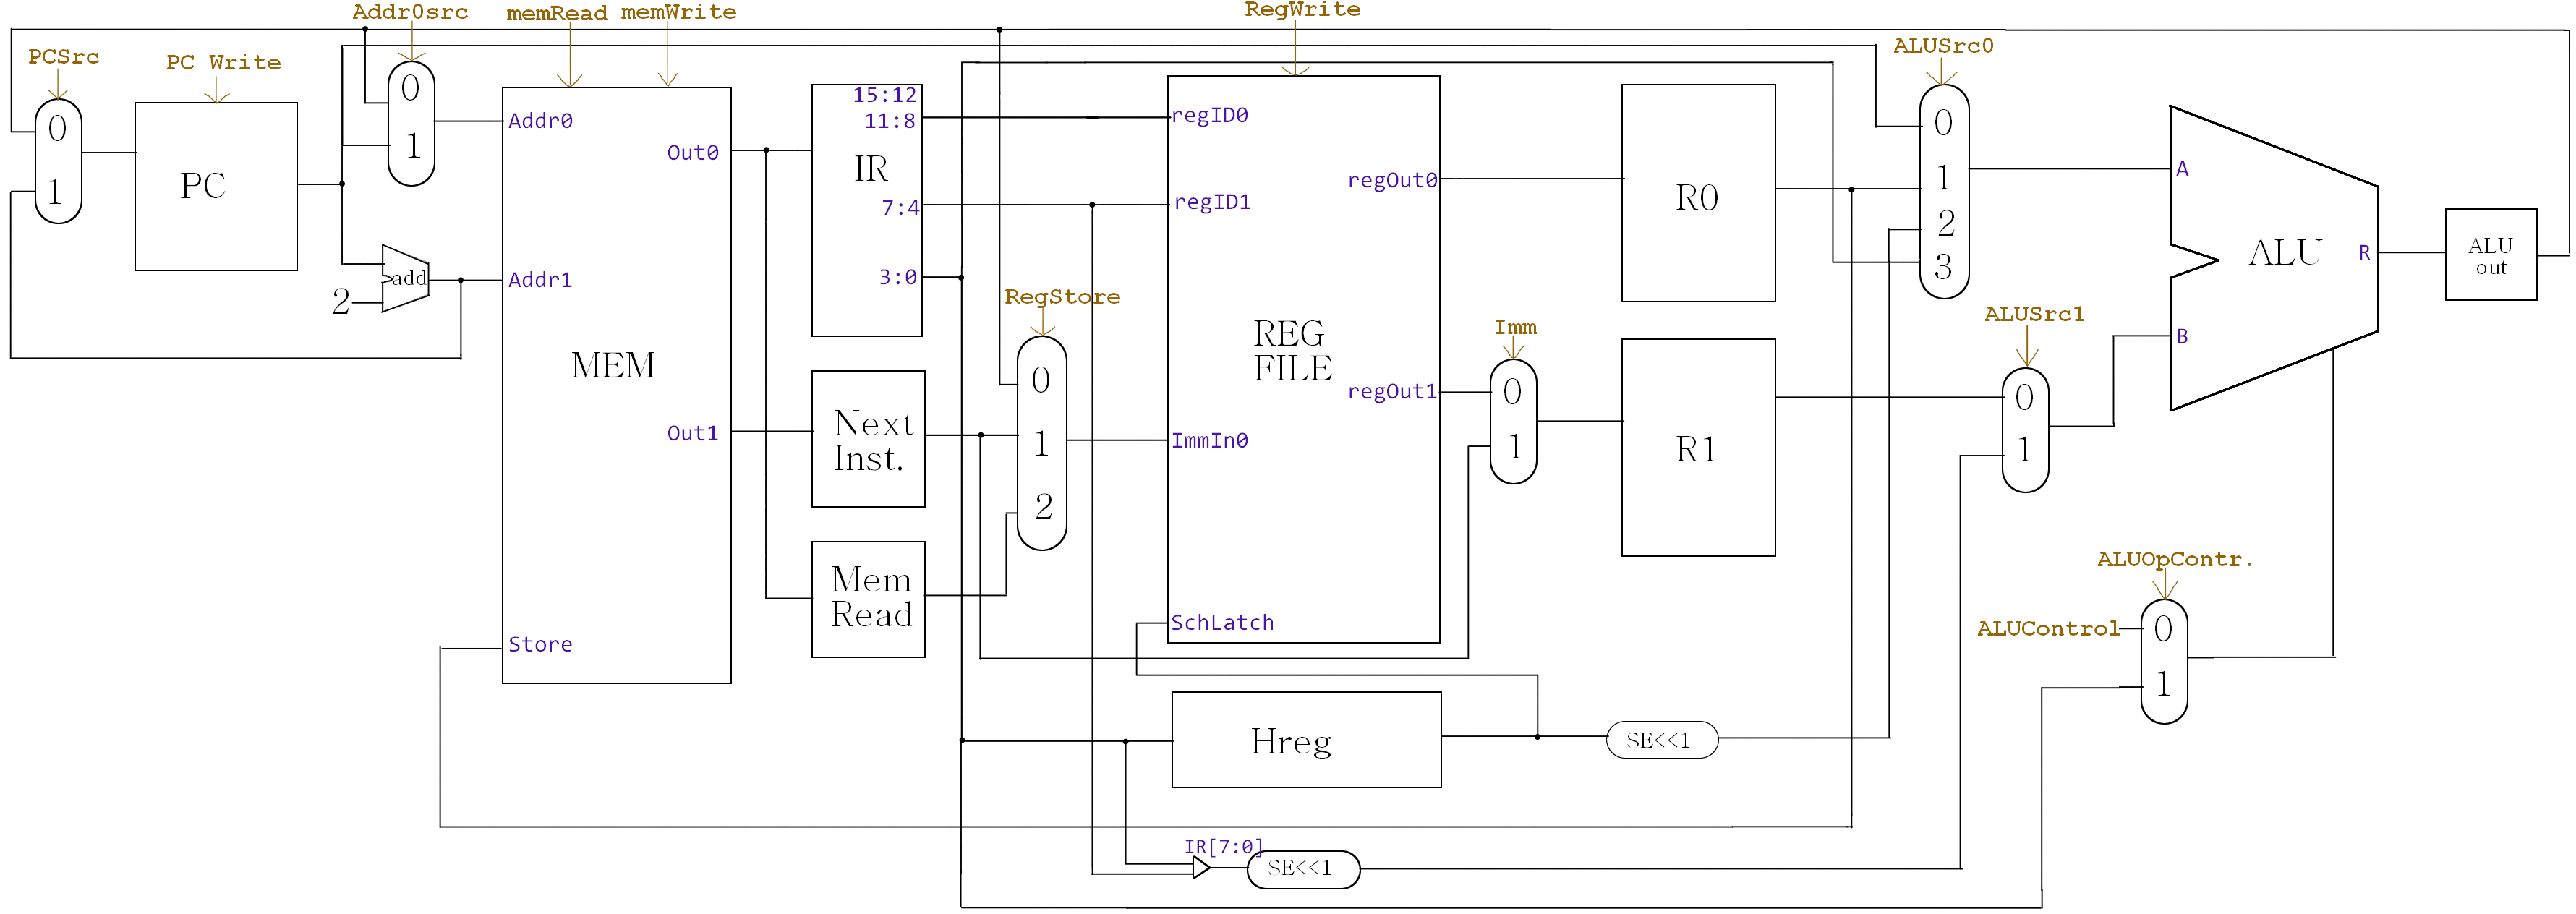
\includegraphics[width=22.25cm]{datapath}
			\end{center} \end{landscape}
	\subsection{Control}
		All of the bits are in hex.  If a control bit is listed below without a value, it is the opposite of it's default. If it is not named, then it is set to it's default, currently, all defaults are 0.
		\begin{center}
			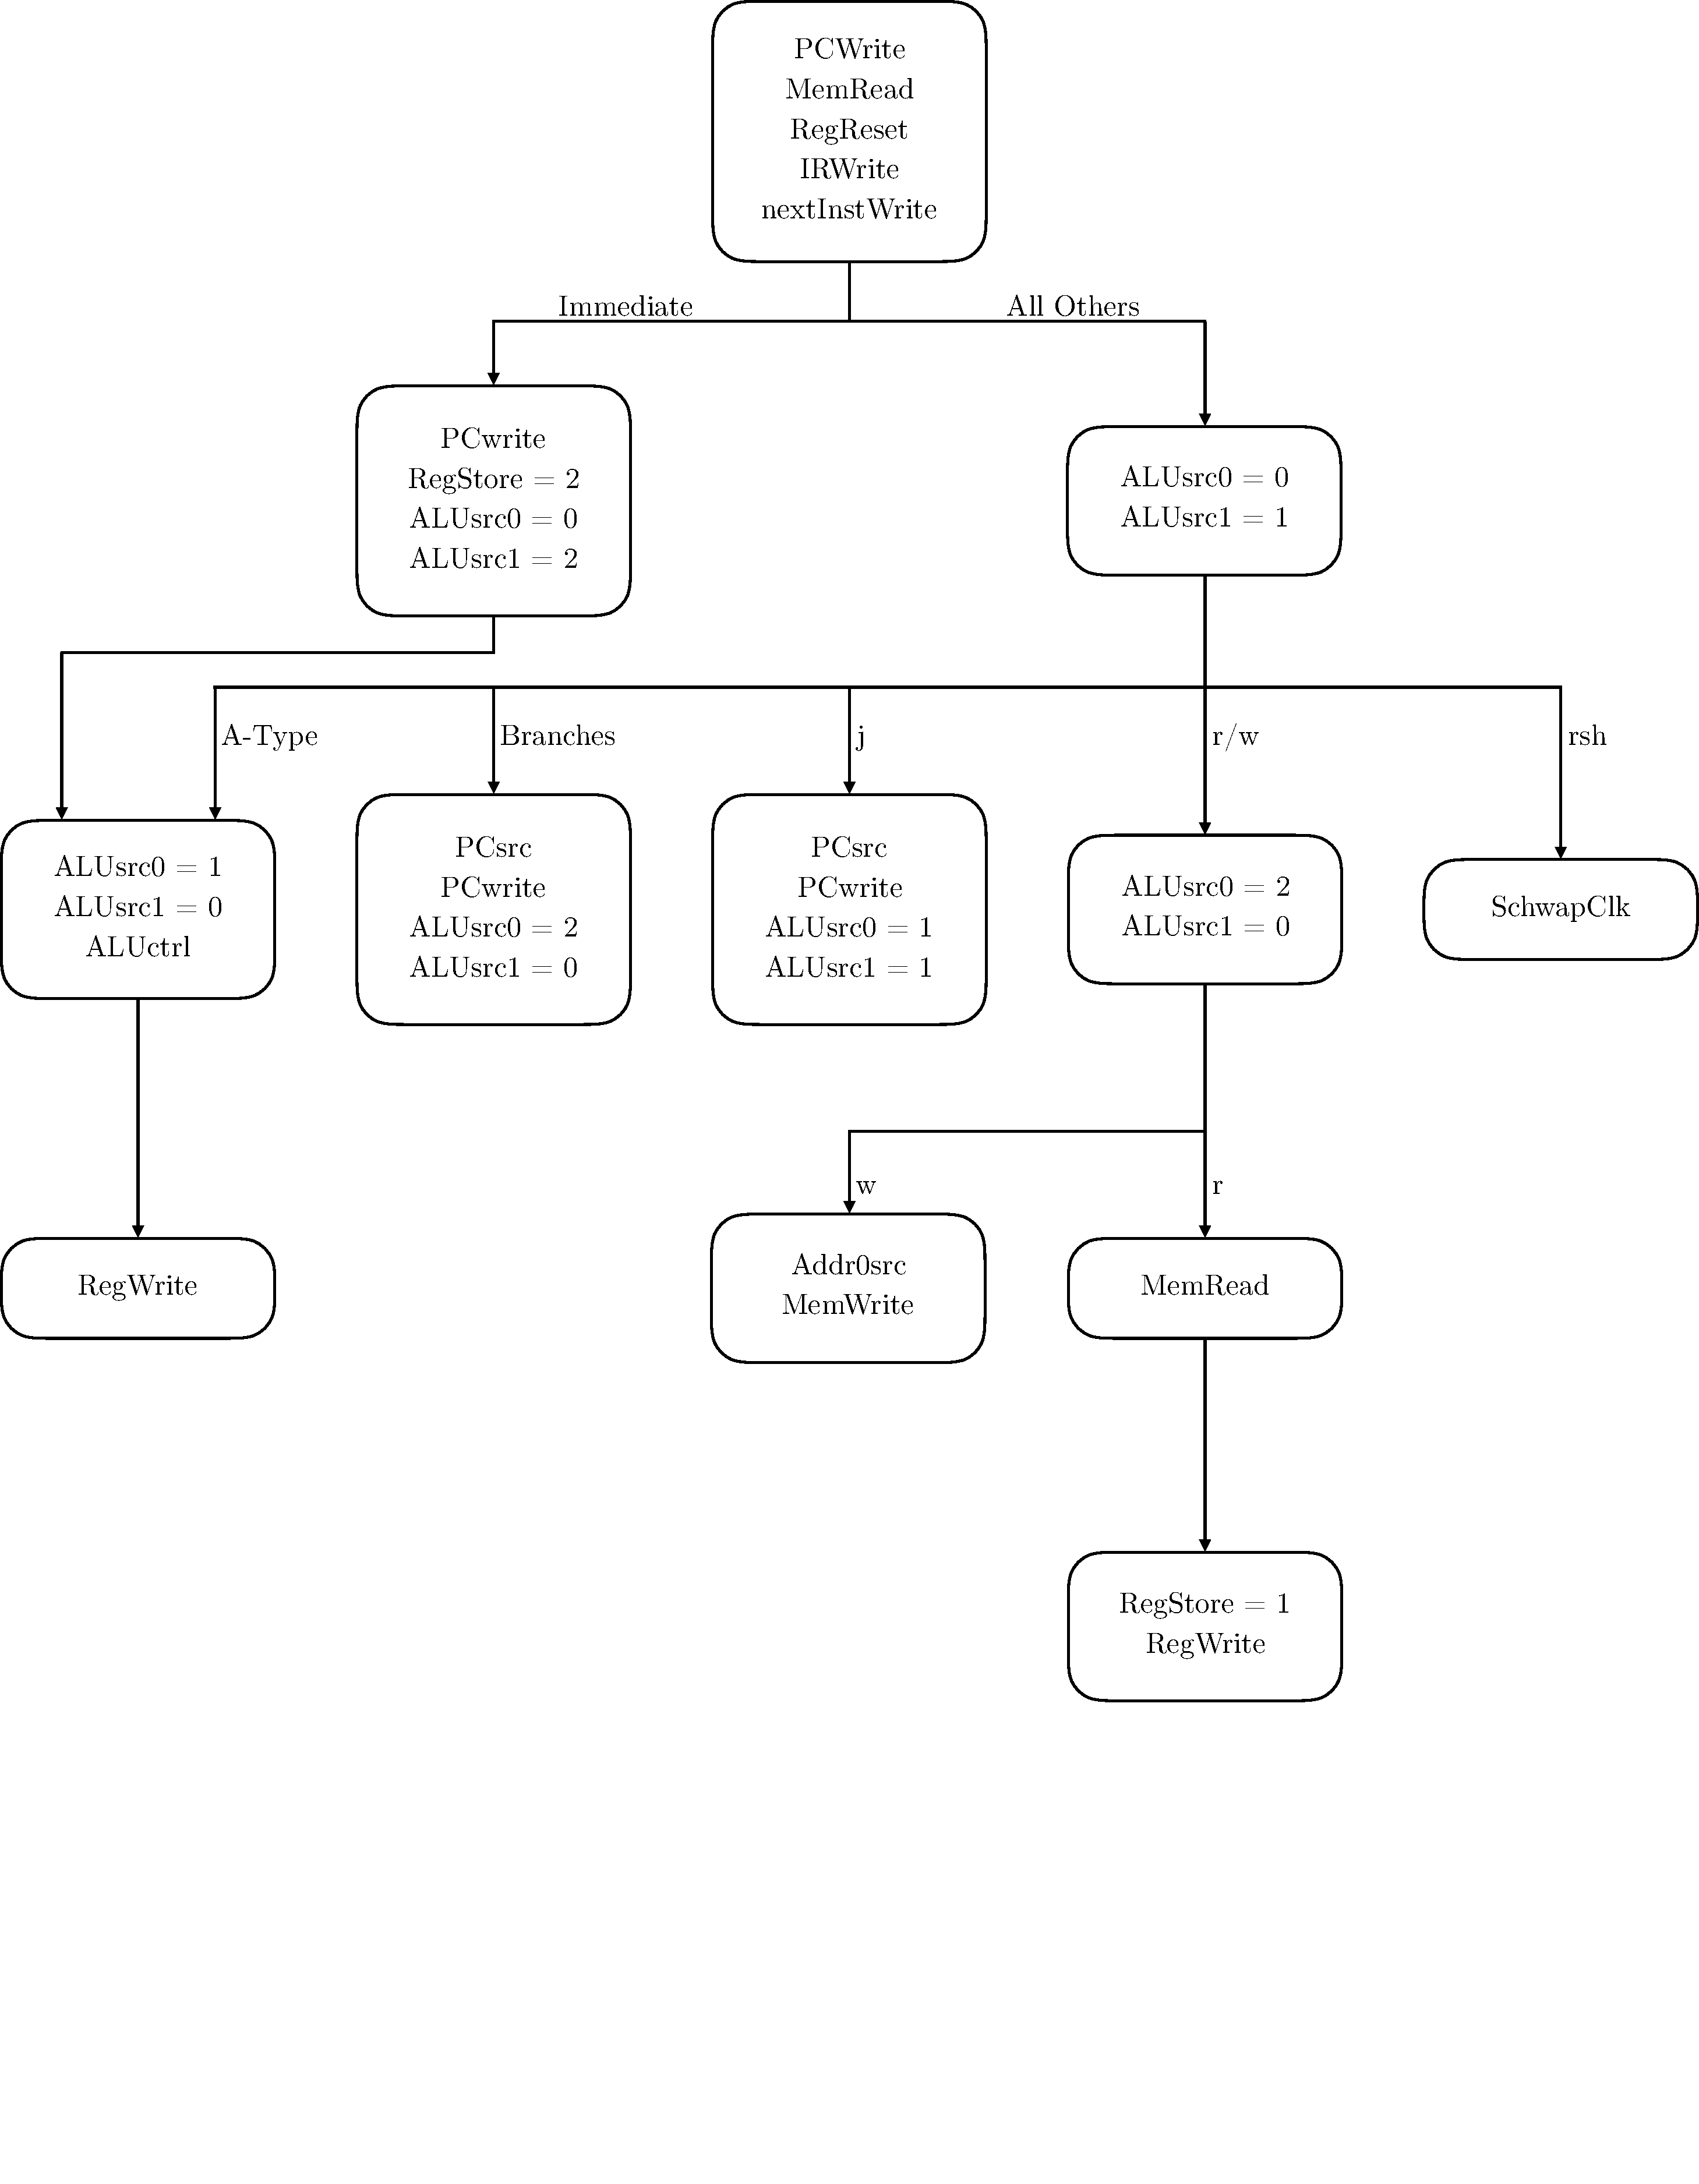
\includegraphics[width=6.25in]{controlSignals}
		\end{center}
	\subsection{Unit Tests and Implementation}
		\subsubsection{Single 16-bit Registers}
			\begin{tabular}{ r  r  p{12cm} }
				Implementation: & \multicolumn{2}{l}{Use Micah's 16 bit register}\\
				                &    & \\
				         Tests: & 1. & Pass in a 16-bit value with writing enabled $\Rightarrow$ The whole value should be stored\\
				                & 2. & Pass in a 16-bit value with writing disabled $\Rightarrow$ The none of the value should be stored\\
			\end{tabular}
		\subsubsection{SE}
			\begin{tabular}{ r  r  p{12cm} }
				Implementation: & \multicolumn{2}{p{12.75cm}}{Split the last wire to make as many more other output bits that are required.}\\
				                &    & \\
				         Tests: & 1. & Pass in a value which has a sign bit of 0 $\Rightarrow$ All new bits should be 0\\
				                & 2. & Pass in a value which has a sign bit of 1 $\Rightarrow$ All new bits should be 1\\
			\end{tabular}
		\subsubsection{16-bit Adder}
			\begin{tabular}{ r  r  p{12cm} }
				Implementation: & \multicolumn{2}{p{12.75cm}}{Use 4 4-bit carry look ahead adders connected together like a ripple adder}\\
				                &    & \\
				         Tests: & 1. & Pass in 0 and 0 $\Rightarrow$ The result should be 0\\
				                & 2. & Pass in 0xFFFF and 0x1 $\Rightarrow$ The result should be 0\\
				                & 3. & Pass in 0x1 and 0xFFFF $\Rightarrow$ The result should be 0\\
				                & 4. & Pass in 0xFFFF and 0xFFFF $\Rightarrow$ The result should be 0xFFFE\\
				                & 5. & Pass in any other 2 values $\Rightarrow$ The result should be the 2 inputs added together\\
			\end{tabular}
		\subsubsection{ALU}
			\begin{longtable}{ r r r p{11cm} }
				Implementation: & \multicolumn{3}{p{12.75cm}}{Use the 16-bit adder above}\\
				                &      &    & \\
				         Tests: & \multicolumn{3}{p{12.75cm}}{Note:  Any time the ALU result is 0, the "zero" output should be 1, all other times it should be 0}\\
				                & and: & 1. & Pass in 0 and 0 $\Rightarrow$ The result should be 0\\
				                &      & 2. & Pass in 0xFFFF and 0xFFFF $\Rightarrow$ The result should be 0xFFFF\\
				                &      & 3. & Pass in 0 and 0xFFFF $\Rightarrow$ The result should be 0\\
				                &      & 4. & Pass in any other 2 values $\Rightarrow$ The result should be the 2 inputs anded together\\
				                & orr: & 1. & Pass in 0 and 0 $\Rightarrow$ The result should be 0\\
				                &      & 2. & Pass in 0xFFFF and 0xFFFF $\Rightarrow$ The result should be 0xFFFF\\
				                &      & 3. & Pass in 0 and 0xFFFF $\Rightarrow$ The result should be 0xFFFF\\
				                &      & 4. & Pass in any other 2 values $\Rightarrow$ The result should be the 2 inputs orred together\\
				                & xor: & 1. & Pass in 0 and 0 $\Rightarrow$ The result should be 0\\
				                &      & 2. & Pass in 0xFFFF and 0xFFFF $\Rightarrow$ The result should be 0\\
				                &      & 3. & Pass in 0 and 0xFFFF $\Rightarrow$ The result should be 0xFFFF\\
				                &      & 4. & Pass in any other 2 values $\Rightarrow$ The result should be the 2 inputs xorred together\\
				                & not: & 1. & Pass in 0 $\Rightarrow$ The result should be 0xFFFF\\
				                &      & 2. & Pass in 0xFFFF $\Rightarrow$ The result should be 0\\
				                &      & 3. & Pass in any other value $\Rightarrow$ The result should be the input notted\\
				                & tsc: & 1. & Pass in 0 $\Rightarrow$ The result should be 0\\
				                &      & 2. & Pass in 0xFFFF $\Rightarrow$ The result should be 0x1\\
				                &      & 3. & Pass in any other value $\Rightarrow$ The result should be the input converted to 2's compliment\\
				                & slt: & 1. & Pass in 0 and 0 $\Rightarrow$ The result should be 0\\
				                &      & 2. & Pass in 0xFFFF and 0xFFFF $\Rightarrow$ The result should be 0\\
				                &      & 3. & Pass in 0xFFFF and 0 $\Rightarrow$ The result should be 0x1\\
				                &      & 4. & Pass in 0 and 0xFFFF $\Rightarrow$ The result should be 0\\
				                &      & 5. & Pass in 2 values such that the first is smaller than the second $\Rightarrow$ The result should be 0\\
				                &      & 6. & Pass in 2 values such that the second is smaller than the first $\Rightarrow$ The result should be 0x1\\
				                & sll: & 1. & Pass in 0 and 0 $\Rightarrow$ The result should be 0\\
				                &      & 2. & Pass in 0xFFFF and 0 $\Rightarrow$ The result should be 0xFFFF\\
				                &      & 3. & Pass in 0xFFFF and 0x1 $\Rightarrow$ The result should be 0xFFFE\\
				                &      & 4. & Pass in 0xFFFF and 0xF $\Rightarrow$ The result should be 0x8000\\
				                &      & 5. & Pass in 0 and 0x1 $\Rightarrow$ The result should be 0\\
				                &      & 6. & Pass in 0 and 0xF $\Rightarrow$ The result should be 0\\
				                &      & 7. & Pass in any other 16-bit value for the first and 4-bit value for the second $\Rightarrow$ The result should be the first input shifted to the left by the amount of the second\\
				                & srl: & 1. & Pass in 0 and 0 $\Rightarrow$ The result should be 0\\
				                &      & 2. & Pass in 0xFFFF and 0 $\Rightarrow$ The result should be 0xFFFF\\
				                &      & 3. & Pass in 0xFFFF and 0x1 $\Rightarrow$ The result should be 0x7FFF\\
				                &      & 4. & Pass in 0xFFFF and 0xF $\Rightarrow$ The result should be 0x1\\
				                &      & 5. & Pass in 0 and 0x1 $\Rightarrow$ The result should be 0\\
				                &      & 6. & Pass in 0 and 0xF $\Rightarrow$ The result should be 0\\
				                &      & 7. & Pass in any other 16-bit value for the first and 4-bit value for the second $\Rightarrow$ The result should be the first input shifted to the right by the amount of the second and the new spots should be filled with 0's\\
				                & sra: & 1. & Pass in 0 and 0 $\Rightarrow$ The result should be 0\\
				                &      & 2. & Pass in 0xFFFF and 0 $\Rightarrow$ The result should be 0xFFFF\\
				                &      & 3. & Pass in 0xFFFF and 0x1 $\Rightarrow$ The result should be 0xFFFF\\
				                &      & 4. & Pass in 0xFFFF and 0xF $\Rightarrow$ The result should be 0xFFFF\\
				                &      & 5. & Pass in 0 and 0x1 $\Rightarrow$ The result should be 0\\
				                &      & 6. & Pass in 0 and 0xF $\Rightarrow$ The result should be 0\\
				                &      & 7. & Pass in 0x7FFF and 0x1 $\Rightarrow$ The result should be 0x3FFF\\
				                &      & 8. & Pass in 0x7FFF and 0xE $\Rightarrow$ The result should be 0x1\\
				                &      & 9. & Pass in 0x7FFF and 0xF $\Rightarrow$ The result should be 0\\
				                &      & 10.& Pass in any other 16-bit value for the first and 4-bit value for the second $\Rightarrow$ The result should be the first input shifted to the right by the amount of the second and the new spots should be filled with the leading digit\\
				                & add: & 1. & Pass in 0 and 0 $\Rightarrow$ The result should be 0\\
				                &      & 2. & Pass in 0xFFFF and 0x1 $\Rightarrow$ The result should be 0\\
				                &      & 3. & Pass in 0x1 and 0xFFFF $\Rightarrow$ The result should be 0\\
				                &      & 4. & Pass in 0xFFFF and 0xFFFF $\Rightarrow$ The result should be 0xFFFE\\
				                &      & 5. & Pass in 0x7FFF and 0x1 $\Rightarrow$ The result should be 0x8000\\
				                &      & 6. & Pass in 0x7FFF and 0x7FFF $\Rightarrow$ The result should be 0xFFFE\\
				                &      & 7. & Pass in any other 2 values $\Rightarrow$ The result should be the 2 inputs added together\\
				                & sub: & 1. & Pass in 0 and 0 $\Rightarrow$ The result should be 0\\
				                &      & 2. & Pass in 0xFFFF and 0x1 $\Rightarrow$ The result should be 0xFFFE\\
				                &      & 3. & Pass in 0x1 and 0xFFFF $\Rightarrow$ The result should be 0x10\\
				                &      & 4. & Pass in 0xFFFF and 0xFFFF $\Rightarrow$ The result should be 0\\
				                &      & 5. & Pass in 0x8000 and 0x1 $\Rightarrow$ The result should be 0x7FFF\\
				                &      & 6. & Pass in 0x8000 and 0x7FFF $\Rightarrow$ The result should be 0x1\\
				                &      & 7. & Pass in any other 2 values $\Rightarrow$ The result should be the 2 inputs subtracted\\
				                & cpy: & 1. & Pass in 0 $\Rightarrow$ The result should be 0\\
				                &      & 2. & Pass in 0xFFFF $\Rightarrow$ The result should be 0xFFFF\\
				                &      & 3. & Pass in any other value $\Rightarrow$ The result should the value\\
			\end{longtable}
		\subsubsection{Schwap}
			\begin{tabular}{ r  r  p{12cm} }
				Implementation: & \multicolumn{2}{p{12.75cm}}{Use 4 16-bit wide schmuxes which switch to 16 16-bit registers each, and then 4 16-bit deschmuxes to each group of the 16 registers}\\
				                &    & \\
				         Tests: & 1. & Set Schlatch to 0 $\Rightarrow$ The schlatch should be set to 0 and should allow reading and writing to schwap group 0\\
				                & 2. & Write values $\Rightarrow$ The values should be written to the group number according to the schlatch\\
					            & 3. & Change schlatch $\Rightarrow$ The values in the previous and new schwap group should not have been altered\\
					            & 4. & Write data to a new schwap group $\Rightarrow$ The data should be written to the new schwap group and the data in the old group should not have been altered\\
					            & 5. & Change back to a previously used schlatch $\Rightarrow$ The data previously written data should still be in the schwap group\\
			\end{tabular}
		\subsubsection{Register File}
			\begin{tabular}{ r  r  p{12cm} }
				Implementation: & \multicolumn{2}{p{12.75cm}}{Create one 16-bit register hard-wired to 0, 11 normal 16-bit registers, and a schwap.}\\
				                &    & \\
				         Tests: & 1. & Pass in 2 register IDs between 0 and 11 into the to regID inputs $\Rightarrow$ The result should be the values in the given registers (regOut0 has the value from regID0 and regOut1 has the value regID1)\\
				                & 2. & Pass in 2 register IDs between 12 and 15 into the to regID inputs $\Rightarrow$ The result should be the values in the given registers (regOut0 has the value from regID0 and regOut1 has the value regID1) and use the correct schwap group\\
				                & 3. & Pass in a number between 0 and 14 to SchLatch $\Rightarrow$ The data coming out of registers 12 - 15 should be from the schwap group number given to SchLatch\\
				                & 4. & Pass in a register ID using regID1 between 0 and 11 with a value to ImmIn0 and RegWrite set to 1 $\Rightarrow$ The result should be stored in the register given on regID1, and regID0 should be ignored\\
				                & 5. & Pass in a register ID using regID1 between 12 and 15 with a value to ImmIn0 and RegWrite set to 1 $\Rightarrow$ The result should be stored in the register given on regID1 in the correct schwap group, and regID0 should be ignored\\
			\end{tabular}
		\subsubsection{Main Memory}
			\begin{tabular}{ r  r  p{12cm} }
				Implementation: & \multicolumn{2}{p{12.75cm}}{Use a Xilnix created memory with 2 address inputs, 2 outputs, and at least 1 write data input}\\
				                &    & \\
				         Tests: & 1. & Pass in 2 valid memory addresses and set the memRead to 1 $\Rightarrow$ The data in at those memory addresses should be output\\
				                & 2. & Pass in data to Store and a valid memory address and set memWrite to 1 $\Rightarrow$ The the data from Store should have been written to memory\\
				                & 3. & Pass in data to Store and a valid memory address and set memWrite to 0 $\Rightarrow$ The the data from Store should not have been written to memory\\
			\end{tabular}
	\subsection{Integration Tests}
		\subsubsection{PC and Memory}
			\begin{tabular}{ r  p{15cm} }
				1. & Set PC to some initial value for testing\\
				2. & Clock PCWrite at least 16 times\\
				3. & Write data to those 16 addresses and set PC to the original value for testing\\
				4. & Clock PCWrite so it will iterate over the values put into memory, also check that the outputs from memory are correct\\
			\end{tabular}
		\subsubsection{Register File and ALU}
			\begin{tabular}{ r  p{15cm} }
				1. & Write test data to each register in the register file\\
				2. & Do operations using the ALU to the values in the register file using every register and ALU op code\\
				3. & Check all of the values in the register file to ensure they are correct\\
			\end{tabular}
	\subsection{System Tests}
		\subsubsection{A-Type}
			\begin{tabular}{ r  r  p{12cm} }
				No Immediate:   & 1. & Get this instruction\\
				                & 2. & Increase PC by 1 for the next instruction\\
				                & 3. & R0 and R1 should be loaded with the values from the first and second register in the instruction\\
				                & 4. & The ALUout should have the value of the two values combined using the function code that was passed in\\
				                & 5. & That value should be in the first specified register for the instruction\\
				                &    & \\
				With Immediate: & 1. & Get this and the next instruction\\
				                & 2. & Increase PC by 1 for the next instruction\\
				                & 3. & R0 should be loaded with the value from the first register in the instruction and R1 should have the immediate which was in NextInst, PC should have been increased by 2 again\\
				                & 4. & The ALUout should have the value of the two values combined using the function code that was passed in\\
				                & 5. & That value should be in the first specified register for the instruction, the immediate should also have been stored in the second register from the instruction if it was given\\
			\end{tabular}
		\subsubsection{B-Type}
			\begin{longtable}{ r  r  p{13cm} }
				Branches: & 1. & Get this instruction\\
				          & 2. & Increase PC by 1 for the next instruction\\
				          & 3. & R0 and R1 should be loaded with the values from the first and second register in the instruction\\
				          & 4. & The ALUout should have the new PC value for use if the branch is supposed to branch\\
				          & 5. & ALUout should be transferred to PCtemp, the combination of R0 and R1 should be in ALUout\\
				          & 6. & If ALUout is 0 PC should have been changed to what is in PCtemp\\
				          &    & \\
				Read:     & 1. & Get this instruction\\
				          & 2. & Increase PC by 1 for the next instruction\\
				          & 3. & R0 and R1 should be loaded with the values from the first and second register in the instruction, Hreg should have the offset from the instruction\\
				          & 4. & The ALUout should have the value of what's in R1 added to the sign extended value in Hreg\\
				          & 5. & ALUout should be passed into main memory and the value at that address should be in MemRead\\
				          & 6. & The first register specified in the instruction should have the value from memory\\
				          &    & \\
				Write:    & 1. & Get this instruction\\
				          & 2. & Increase PC by 1 for the next instruction\\
				          & 3. & R0 and R1 should be loaded with the values from the first and second register in the instruction, Hreg should have the offset from the instruction\\
				          & 4. & The ALUout should have the value of what's in R1 added to the sign extended value in Hreg\\
				          & 5. & ALUout should be passed into memory as well as the value in R0, the value in R0 should be in memory at that address
			\end{longtable}
		\subsubsection{H-Type}
			\begin{tabular}{ r  r  p{12cm} }
				Schwap: & 1. & Get this instruction\\
				        & 2. & Increase PC by 1 for the next instruction\\
				        & 3. & Hreg should get the schwap group number\\
				        & 4. & SchLatch should now be set to the new schwap group number\\
				        &    & \\
				Sudo:   & 1. & Get this instruction\\
				        & 2. & Increase PC by 1 for the next instruction\\
				        & 3. & Hreg should get the sudo code number\\
				        & 4. & The correct action should now be performed based on the code number\\
				        &    & \\
				Spc:    & 1. & Get the PC value\\
				        & 2. & Increment PC\\
				        & 3. & Switch to spc\\
			\end{tabular}
		\subsubsection{J-Type}
			\begin{tabular}{ r  r  p{12cm} }
				jr: & 1. & Get this instruction\\
				    & 2. & Increase PC by 1 for the next instruction\\
				    & 3. & PC should be changed to the value in R0 added to the sign extended value in IR[7:0]\\
			\end{tabular}
\section{Coding Practices}
	\begin{enumerate}
		\item Programs should always be ended with "sudo 0".
		\item Avoid branching up and more than 16 instructions down.  The hardware implementation of branching limits branching to only going down a maximum of 16 instructions, but the assembler will convert these to a combination of a branch and jump.
		\item Schwap groups are not preserved across calls, including sudo calls.
	\end{enumerate}
\section{Assembler}
	\subsection{Using the Assembler}
		Calling the program: "assembler infile.asm $<$outfile.bin$>$ $<$Program Start offset$>$ $<$debug$>$"
		\begin{itemize}
			\item Use the "-h" flag to display help
			\item If the outfile is not specified, it will write to out.bin
			\item If 'debug'(all lowercase) is passed anywhere, it will toggle debugging mode
			\item If an integer (in decimal) is passed, it will offset the program counter so that all direct jumps are recorded accurately, it defaults to 4096(or 0x1000).  This is highly recommended, do not touch unless you know what you are doing.
		\end{itemize}
	\subsection{Supported Pseudo Instructions}
		\begin{tabular}{ r p{1cm} p{15cm} }
			jal: & \multicolumn{2}{ p{15cm} }{Jump and link.  It will set RA to the PC after this instruction call.  It takes a label.}\\
				 & & Example:  jal label \\
				 & \\
			j:   & \multicolumn{2}{ p{15cm} }{Jumps to a label.  This instruction is extended to jr \$pc label.} \\
				 & & Example:  j label \\
				 & \\
			psh: & \multicolumn{2}{ p{15cm} }{Push.  Decrease the stack pointer by 1 and push a value in a register to the user stack.} \\
				 & & Example: psh \$t0 \\
				 & \\
			pop: & \multicolumn{2}{ p{15cm} }{Pop. Reads a value from the stack and add 1 to the stack pointer.} \\
				 & & Example:  pop \$t0 \\
				 & \\
			nop: & \multicolumn{2}{ p{15cm} }{No Operator.  Becomes and \$0 \$0.} \\
				 & & Example:  nop \\
				 & \\
			bge: & \multicolumn{2}{ p{15cm} }{Branch if Greater Than or Equal To.  Branch to a label if the value in register one is grater than or equal to the value in the second register.} \\
				 & & Example:  bge $t0 $t1 label\\
				 & \\
			ble: & \multicolumn{2}{ p{15cm} }{Branch if Less Than or Equal To.  Branch to a label if the value in register one is less than or equal to the value in the second register.} \\
				 & & Example:  bge $t0 $t1 label\\
		\end{tabular}
	\subsection{Supported Shortcuts}
		\subsubsection{Schwap}
			All instructions that use schwap registers can use the notation \$hn@m where \$hn is the target schwap register, and m is the target schwap group.  This can be used if one or both registers are schwap.  This should work with all instructions, but has only been throughly tested with ALU operations.  These are not dependent on the position of the register in the instruction.\\
			\begin{tabular}{ r  p{0.5cm}  p{12cm} }
						   & & \\
				Example 1: & & add \$h0@5 \$t0 \\
						   & \multicolumn{2}{ l }{Is translated to} \\
						   & & rsh 5 \\
						   & & add \$h0 \$t0 \\
						   & & \\
				Example 2: & & slt \$h0@5 \$h0@8 \\
						   & \multicolumn{2}{ l }{Is translated to} \\
						   & & rsh 8 \\
						   & & cpy \$a0 \$h0 \\
						   & & rsh 5 \\
						   & & slt \$h0 \$a0 \\
			\end{tabular}
	\subsection{Adding Pseudo Instructions}
		If you REALLY want to add pseudo instructions, there is documentation within the Python file.  Remember to both add the instruction to the PseudoList at the top of the file, and to add the case in pseudoExpandHelper.  Follow the patterns given.  Any modification to the assembler code voids all warranty.
\section{Emulator}
	The emulator can be run from the executable jar, JScpim.jar. Load the kernel and the program into memory. The kernel should be loaded at 0x0000, and the program to be run should be loaded at 0x1000.  The file structure it takes is as follows. The file may optionally start with a hash sign and a 4-digit hex number. If not, \#1000 is assumed. This is the location the memory will be loaded into.  Memory is taken in the form "0xHHHH", where H is a hex digit. Each 16-bits of memory should be on its own line. Invalid lines will be ignored.\par
	The emulator is slightly buggy, however basic things should work. Note that behavior for minimizing then unminimizing the window is... undefined. Behavior should be normal for using ALT+Tab to switch to/from the window, however, based on the way java handles events.\\
	\begin{center}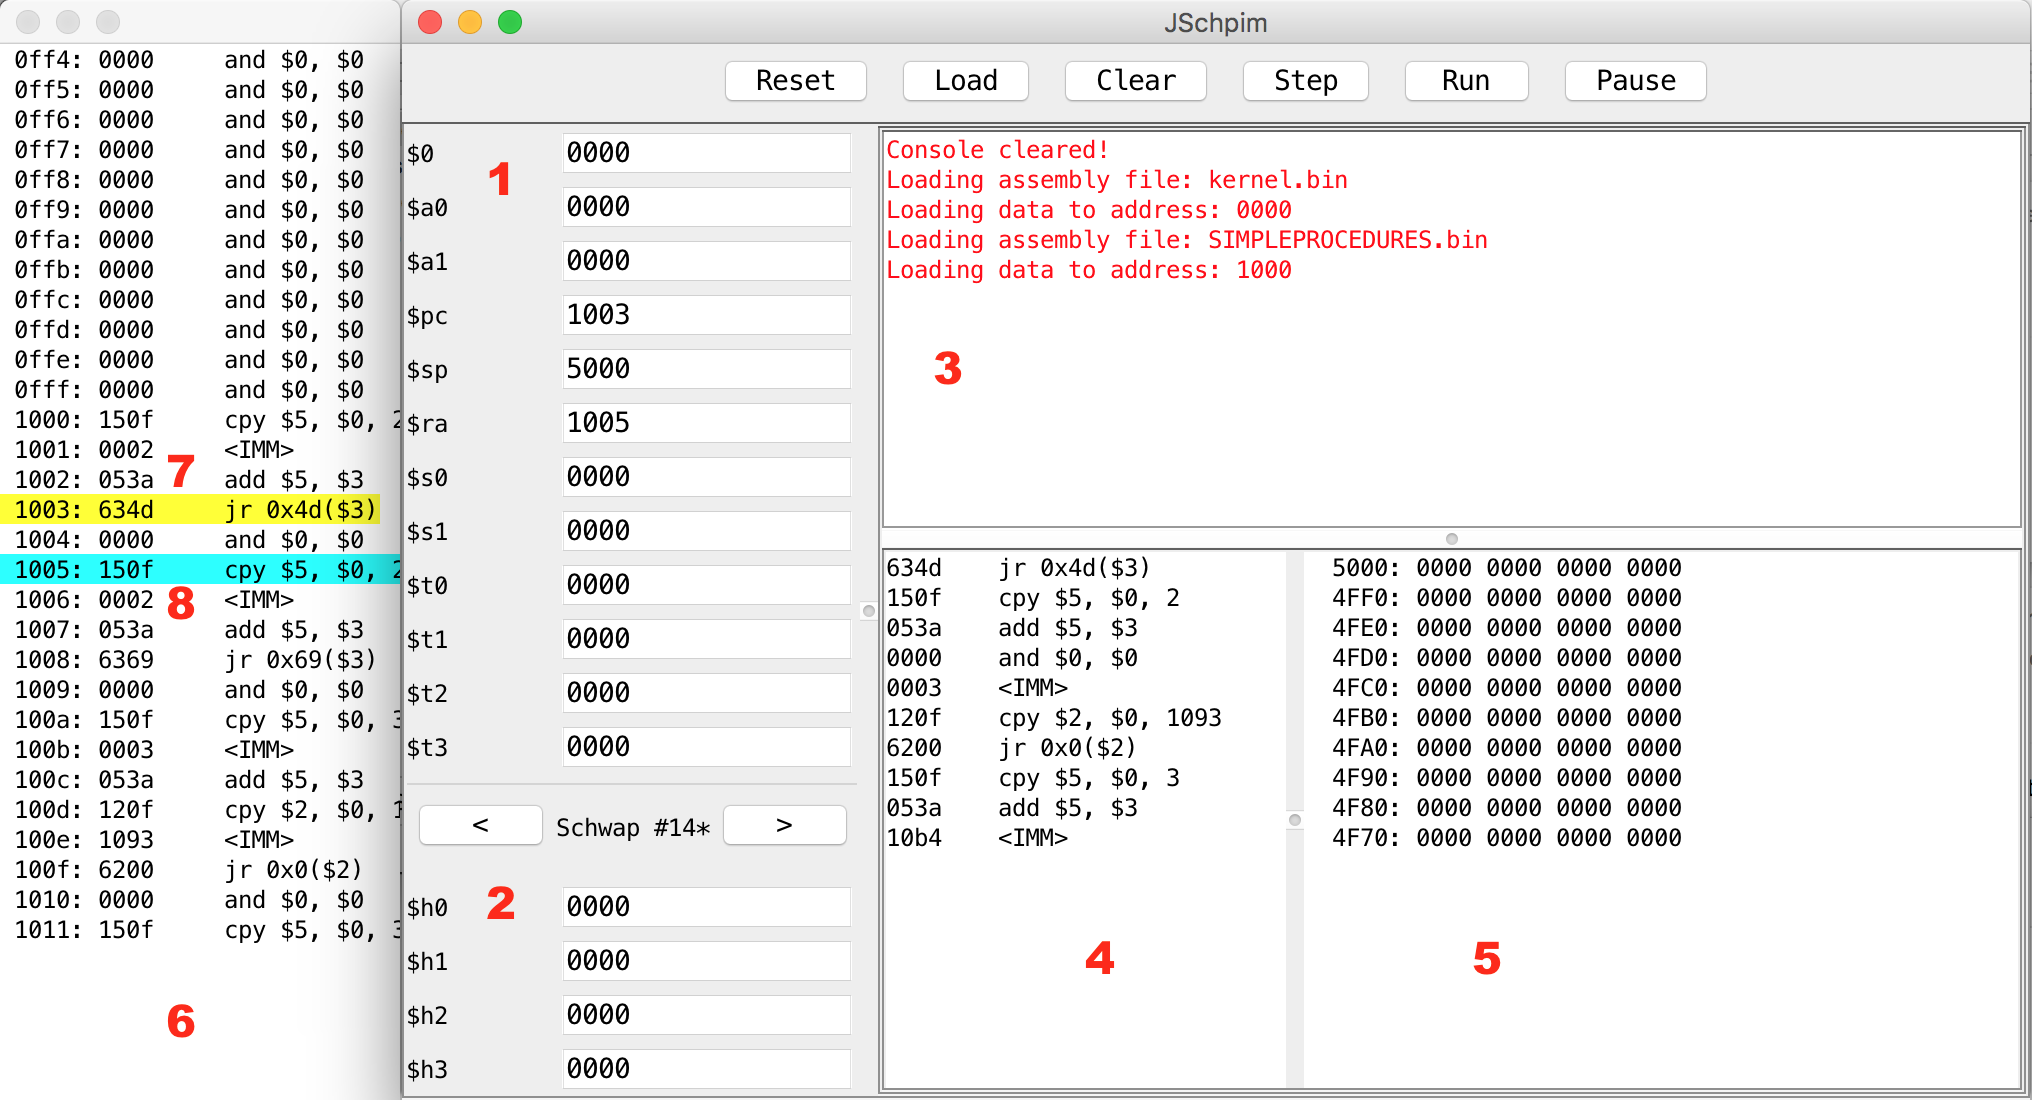
\includegraphics[width=16cm]{jSchpim}\end{center}
	\begin{tabular}{ r l }
		1. & Register contents \\
		2. & Schwap contents \\
		3. & Console output \\
		4. & Current instructions \\
		5. & Stack contents \\
		6. & Debug viewer \\
		7. & Current instruction highlighted in yellow \\
		8. & Instruction pointed to by \$ra highlighted in cyan \\
	\end{tabular}
	\subsection{Known Bugs}
		\begin{itemize}
			\item If you try to become a professional Korean starcraft player on the reset button, the window will break
			\item The illuminati seem to have infiltrated parts of the code base. Don't listen to their lies
			\item It's java and swing... There's going to probably be a lot of bugs but if you're not stupid and/or trying to break it you shouldn't really run into that many
		\end{itemize}
\section{LINUKS}
The Kernel (LINUKS) handles the initialization of the CPU, sudo calls, and exception handling. The kernel is always loaded starting at 0x0000. Instructions 0x0001 to 0x000F should jump to the sudo handlers for the same number as the address (e.g. 0x0001 should be a 16-bit jump to the sudo 1 handler).  The initialization of the CPU includes waiting for 1,000,000 cycles @ 50MHz, setting the \$sp=0xFFFF, and jumping to 0x1000 where the program is loaded.  The 1,000,000 cycles are representative of the amount of 50Hz cycles it would take LCD to initialize if it were implemented in the future.  Sudo calls are outlined in section 2.2.2. While all the ones mentioned are currently implemented, the rest remain reserved for unspecified future use, and will do nothing if called.  Exceptions are handled by jumping to 0x0000. Rather than performing sudo 0, which is dealt with in hardware, it will jump to the exception handler. Currently interrupts and exceptions will not occur naturally. However, we decided to include it so that programmer-defined exception handling was possible.
\section{Program Loader}
	\subsection{Using the Program Loader}
		Calling the loader:  programLoader program.bin <memory.coe> <kernel.bin>\\
		Data can be preloaded into the memory file by adding "loc = data" to the end of the assembly
		\begin{itemize}
			\item loc being the exact location (in decimal) above the program and below 15480 (15480 to 20480 is user stack, can use but be careful) and above 10000 or the end of your program, your decision
			\item data is a 4 digit hex number, must be at most 4 digits, in hex.  Also, please augment with zeroes, not doing so is untested because coe files are weird.
			\item Example:  10101 = abcd
		\end{itemize}
		There is not a lot of checking in this code, if it fails, it's on you.  These are the ranges for memory:
		\begin{center} \begin{tabular}{ r l }
			kernel code & [0:4096) \\
			user code   & [4096:10000) \\
			user space  & [10000:15480) \\
			stack       & [15480:20480] \\
		\end{tabular} \end{center}
\section{The C$\flat$ Programming Language and compiler}
	The C$\flat$ Programming Language is mostly just a watered down version of C and it is a Turing Complete programming language.
	\subsection{Supported Features}
		\subsubsection{Data Types}
			Currently, the only supported data type is a 16-bit signed integer, which is called "int".
		\subsubsection{Scope}
			Scope is contained the same way in C$\flat$ as it is in C, with "\{" and "\}" to open and close the current scope respectively.
		\subsubsection{Operators}
			Operators for combining values and variables:
			\begin{center} \begin{tabular}{| l | p{10cm} |} \hline
				Syntax & Description \\ \hline
				$+$    & Adds the values on either side\\ \hline
				$-$    & Subtracts the values on either side\\ \hline
			\end{tabular} \end{center}
			Operators for comparing values and variables:
			\begin{center} \begin{tabular}{| l | p{10cm} |} \hline
				Syntax & Description \\ \hline
				$==$   & Checks if the values on either side are the same\\ \hline
				$!=$   & Checks if the values on either side are the different\\ \hline
				$>$    & Checks if the value on the left side is greater than the value on the right side\\ \hline
				$>=$   & Checks if the value on the left side is greater than or equal to the value on the right side\\ \hline
				$<$    & Checks if the value on the left side is less than the value on the right side\\ \hline
				$<=$   & Checks if the value on the left side is less than or equal to the value on the right side\\ \hline
			\end{tabular} \end{center}
		\subsubsection{Declaring and assigning variables}
			Variable names should always start with letters and never contain spaces.  Declaring a variable can use any of the following syntaxes:\\
			\begin{center} \begin{tabular}{| l | p{10cm} |} \hline
				Syntax     & Description \\ \hline
				int a;     & Reserves a place in memory/registers for the variable "a"\\ \hline
				int a, b;  & Reserves places in memory/registers for the variables "a" and "b", this can pattern can be expanded to declare as many variables as desired\\ \hline
				int a = 5; & Reserves a place in memory/registers for the variable "a" and then sets it to the value $5$\\ \hline
			\end{tabular} \end{center}
			Assigning variables can be done with any of the following syntaxes:\\
			\begin{center} \begin{tabular}{| l | p{10cm} |} \hline
				Syntax        & Description \\ \hline
				a = 5;        & Sets the variable "a" to $5$\\ \hline
				a = b + 5;    & Sets the variable "a" to "b" $+$ $5$, the $+$ can be any valid combining operator\\ \hline
				a = b + c;    & Sets the variable "a" to "b" $+$ "c", the $+$ can be any valid combining operator\\ \hline
				a += 5;       & Adds $5$ to the variable "a", the $+$ can be any valid combining operator\\ \hline
				a = method(); & Sets the variable "a" to the return value of "method"\\ \hline
			\end{tabular} \end{center}
		\subsubsection{Conditionals}
			Opening an if statement should use the following syntax, "if (x $==$ y) \{", where x and y are variables, constants, or any mix of the two. The "$==$" can be any conditional operator. Closing an if should have either a "\}", use the else if syntax, or the else syntax.  Else if statements should use the the following syntax "\} elif (x $==$ y) \{", where x and y are variables, constants, or any mix of the two.  The "$==$" can be any conditional operator and the keyword "elif" can also be "else if".  The else if statements should be closed with a "\}" or have an else statement following it.  Else statements should use the syntax "\} else \{" and then be closed with "\}".  These statements can be nested within each other or loops.
		\subsubsection{Loops}
			Starting a while loop should use the following syntax, "while (x $==$ y) \{", where x and y are variables, constants, method calls or any mix of the three. The "$==$" can be any conditional operator.  The while loop should be closed with a "\}".  While loops can be nested inside of other loops and conditionals.
		\subsubsection{Methods}
			Defining a method can be done anywhere in the file without anything saying its defined (e.g. in C you must do something like "int method();" before adding the method itself).  A method definition should be started with "int nameOfMethod(int arg0, int arg1, int arg2, int arg3) \{", where the first "int" is the return variable type, "nameOfMethod" is the method name (these should never be duplicated in a file or contain spaces).  Inside the parentheses are the 4 arguments, these are optional, the "int" part of each of them is the variable type and "arg" with a 0, 1, 2, or 3 after it is the variable name that the argument will take.  Methods should always have a return.  They should use the following syntax and can be used anywhere in the method.  "return a, b, c, d;" where "a", "b", "c", and "d" are variables or constants, there can be between 1 and 4 returned values (1 return value would use the syntax "return a;").  Although returning 4 values is supported, it is currently not supported assigning more than the first value in the return.  Methods should be called with the syntax "nameOfMethod(arg0, arg1)", where "nameOfMethod" is the name of the method to be called and "arg0" and "arg1" are arguments, there can be between 0 and 4 arguments and there should be as many as the method being called requires.  A method can be called before it is defined as long as it is defined somewhere in the file.
	\subsection{Known bugs and glitches}
		\begin{enumerate}
			\item Once the temp registers are all used it breaks because it has not been added to put things on and pull things off of the stack.
			\item There is no syntax checker.  If something is not stated in this documentation it may or may not work as intended.
			\item Multiple lines cannot be put on one line using semicolons.
		\end{enumerate}
\section{Examples}
	\lstset{language=sh}
	\subsection{Loading an immediate into a register}
		\begin{multicols}{2}
			\begin{lstlisting}[frame=single]
cpy $t0 32	# Loads 32 into t0
			\end{lstlisting}
		\columnbreak
			\begin{lstlisting}[frame=single]
0x180f
0x0020
			\end{lstlisting}
		\end{multicols}
	\subsection{Making a Procedure Call}
		\begin{multicols}{2}
			\begin{lstlisting}[frame=single]
rsh 8		# Args schwap
cpy $h0 $t0	# Put argument0 in
cpy $h1 $s1	# Put argument1 in
# Store any wanted temps somewhere
jal Call
rsh 9		# Returns schwap
cpy $s0 $h0	# Return value
			\end{lstlisting}
		\columnbreak
			\begin{lstlisting}[frame=single]
0xe008
0x0c8f
0x0d6f
0x150f
0x0001
0x053a
0x63f9
0xe009
0x06cf
			\end{lstlisting}
		\end{multicols}
	\newpage
	\subsection{Iteration and Conditionals}
		This is an example of which will iterate over 4 array elements in memory and add 32 to each of them.  It will stop repeating after the 4 elements using beq.
		\begin{multicols}{2}
			\begin{lstlisting}[frame=single]
# There is a base memory address
# for an array in memory at s0
cpy $t0 8
cpy $t1 $z0
loop:
r   $t2 0($s0)
add $t2 32
w   0($s0) $t2
add $t1 2
beq $t0 $t1 loop
			\end{lstlisting}
		\columnbreak
			\begin{lstlisting}[frame=single]
0x180f
0x0008
0x090f
0x76a0
0x1a0a
0x0020
0x86a0
0x190a
0x0002
0x3891
0x63f8
			\end{lstlisting}
	\end{multicols}
	\subsection{relPrime}
		\begin{multicols}{2}
			\begin{lstlisting}[frame=single]
RELPrime:
	rsh 4
	cpy $h0 $ra
	rsh 8
	cpy $s0 $h0
	cpy $s1 2
RELPrimeWhile:
	rsh 8
	cpy $h0 $s0
	cpy $h1 $s1
	jal GCD
	rsh 9
	cpy $t0 1
	beq $h0 $t0 RELPrimeRet
	add $s1 1
	j RELPrimeWhile
RELPrimeRet:
	rsh 9
	cpy $h0 $s1
	rsh 4
	jr $h0 0
			\end{lstlisting}
		\columnbreak
			\begin{lstlisting}[frame=single]
0xe004
0x0c5f
0xe008
0x06cf
0x170f
0x0002
0xe008
0x0c6f
0x0d7f
0x150f
0x0001
0x053a
0x630b
0xe009
0x180f
0x0001
0x2c83
0x170a
0x0001
0x63f2
0xe009
0x0c7f
0xe004
0x6c00
			\end{lstlisting}
		\end{multicols}
	\newpage
	\subsection{gcd}
		\begin{multicols}{2}
			\begin{lstlisting}[frame=single]
GCD:
	rsh 8
	beq $h0 $0 GCDReturn
GCDWhile:
	beq $h1 $0 GCDReturn
	bgt $h0 $h1 GCDif
GCDelse:
	sub $h1 $h0
	j GCDWhile
GCDif:
	sub $h0 $h1
	j GCDWhile
GCDReturn:
	rsh 8
	cpy $t0 $h0
	rsh 9
	cpy $h0 $t0
	jr $ra 0
			\end{lstlisting}
			\columnbreak
			\begin{lstlisting}[frame=single]
0xe008
0x2c06
0x2d05
0x4cd2
0x0dcb
0x63fc
0x0cdb
0x63fa
0xe008
0x08cf
0xe009
0x0c8f
0x6500
			\end{lstlisting}
		\end{multicols}
\section{Notes}
	\subsection{Registers}
		\subsubsection{Non-Schwappable}
			\begin{enumerate}
				\item \$z0 is reset on the rising edge of each CPU cycle, so it can be used for cycle-temporary storage.
				\item The value in \$pc should always be what the current instruction address is +1.
			\end{enumerate}
	\subsection{Alias names}
		\subsubsection{Registers}
			All registers can be called directly by their ID's in hex or decimal (e.g. \$h0, \$c, and \$12 can all be used)
			\begin{itemize}
				\item[\$z0:] \$0, \$00, \$zz, \$zero
			\end{itemize}
		\subsubsection{Instructions}
			\begin{itemize}
				\item[orr:] or
				\item[bne:] bnq
			\end{itemize}

\chapter{Design Journal}
	\section{Milestone 1}
		In this milestone we accomplished the following:
		\begin{itemize}
			\item Decided on CPU Architecture, Load-Store
			\item Decided on CPU Instruction set basics
			\begin{itemize}
				\item ALU instructions use the first source as the Destination
				\item There is a set of registers that is swappable, henceforth know as Schwappable Registers.
			\end{itemize}
			\item Wrote Assembly instructions for RelPrime
		\end{itemize}
		Alex and Wesley worked on the design of the CPU and Instruction set. Wesley created the documentation and Charlie scribed and provided arguments and counter arguments for ideas.  Andrew didn't show up or reply to emails.
	\section{Milestone 2}
		In this milestone we accomplished the following:
		\begin{itemize}
			\item Implemented recommendations from previous milestone
			\item Started design of components
			\begin{itemize}
				\item Created rough outline of the ALU on a whiteboard
				\begin{itemize}
					\item Created 4-bit carry look ahead adder in Verilog
				\end{itemize}
				\item Figured out how our "SchwapBox" will be implemented
			\end{itemize}
			\item Created RTL
		\end{itemize}
		Our primary meeting was on Sunday the 17th.  We also had more, smaller meetings throughout the week.  During meetings we all contributed to what we were discussing, which were primarily the RTL summary table, SchwapBox, and ALU.  Outside of the meetings Alex primarily worked on the assembler and almost finished it.  Andrew was also experimenting with an assembler, then implemented the 4-bit carry look ahead adder in Verilog and wrote test cases for it.  Wesley did all of the documentation and journal.
	\section{Milestone 3}
		In this milestone we accomplished the following:
		\begin{itemize}
			\item Updated documentation based on recommendations from the previous milestone
			\item Designed data path
			\begin{itemize}
				\item Created data path without control on white board
				\item Added inputs from control elements
				\item Copied whiteboard into FireAlpaca to make it a convenient .PNG
			\end{itemize}
			\item Assembler is working and mostly bug free
			\item Compiler is in progress
			\item Emulator is in progress
		\end{itemize}
		We met Wednesday to work on homework and finish the assembler. A larger meeting took place Sunday to design the data path and finish up other work. Wesley finished about half of a compiler, did the documentation and tests, as well as provided markers and beautiful whiteboard drawing skills. Alex polished off the assembler. Charlie turned the data path into a useful picture, and did the journal. Andrew began progress on the emulator and is about halfway done. Alex, Charlie and Wesley designed the data path on the white board collaboratively.
	\section{Milestone 4}
		In this milestone we accomplished the following:
		\begin{itemize}
			\item Updated documentation based on recommendations from the previous milestone
			\item Created what the control unit should be outputting for what cycle
			\begin{itemize}
				\item Also have a draft of the control unit in Verilog
			\end{itemize}
			\item Integration tests started in Verilog
			\item Assembler was rewritten
			\item Compiler is in progress
			\item Emulator is working
		\end{itemize}
		We had our normal 12ish hour meeting on Sunday to work on the control unit for milestone 4.  Wesley made more progress on compiler, did the documentation, and journal.  Alex rewrote the assembler and started writing integration tests in Verilog.  Charlie put the control unit into Verilog. Andrew now has a working emulator called jSchpim, it has a similar (but better) interface to qtSpim.
	\section{Milestone 5}
		In this milestone we accomplished the following:
		\begin{itemize}
			\item Updated the design docs based on recommendations
			\item Updated the control unit for the changes that we made to the datapath
			\item Updated the Datapath for slight optimizations and to remove extraneous registers
			\item Implemented the separate components and created tests for each set
			\item Finished the assembler worked on the emulator and compiler
			\item Fixed the Verilog code so that the RTL can be synthesized
			\item attached everything together and we are currently working on debugging.
		\end{itemize}
		We had our regular Sunday meeting and finished most of the separate implementation and then spend Monday to Wednesday attaching everything together. Alex finished writing the Assembler and the Memory/PC/Regfile part of the CPU, Charlie finished the control unit, Andrew updated and worked on the assembler as well as finished the ALU, and Wesley worked on the documentation and compiler, which is almost able to compile relPrime and gcd.
	\section{Milestone 6}
		In this milestone we accomplished the following:
		\begin{itemize}
			\item Updated the design docs based on recommendations
			\item Updated the control unit for the changes that we made to the datapath
			\item Updated the Datapath
			\item Tested and debugged CPU
			\item Created a kernel
			\item Put the complier in a state where it can compile relPrime (hopefully correctly)
			\item Started IO
		\end{itemize}
		We had our regular 12 hour meeting on Sunday to start with debugging the CPU and then also had a meeting Tuesday to try and finish up debugging.  Alex and Charlie primarily worked on debugging the CPU.  Andrew worked on ALU debugging and worked on IO as well as writing LINUCKS.  Wesley worked on the compiler as well as doing some documentation updates and journal.
\chapter{Test Results}
	Passing - see final results (Section 1.3.5).
\end{document}
